%!TEX root = ../final-report.tex
\chapter{Implementation}
\label{ch:implementation}

This chapter outlines how the methods derived in the previous section were implemented and evaluated. First, the software package which was used is introduced briefly. Afterwards, the chapter focuses on the framework the author wrote in order to validate and assess the different methods.

\section{Clawpack}

The methods presented in the previous chapter have been implemented using the software package \emph{Clawpack}\footnote{\url{http://www.clawpack.org/}} (\textbf{C}onservation \textbf{law} \textbf{pack}age), version 5.2.2, or more specifically its \emph{Pyclaw} package. Clawpack was originally written by Randall J. LeVeque and is now maintained and further developed by a small group of researchers (including LeVeque).

The basic principle of Clawpack is that the user writes a Riemann solver, which receives the grid of cell averages along with optional auxiliary data and calculates the fluctuations (Eqs.~\ref{eq:fluctuations}) for each cell. The package then uses this to implement Godunov's method in wave propagation form, Eq.~\ref{eq:wpf}. The parameters of the solver, like the grid size, boundary conditions, gravity or the strength of the Coriolis force, as well as the initial conditions and auxiliary data like bathymetry can specified separately. Clawpack also provides the option to specify a separate function to be solved after each time step which can be used to implement source terms via source splitting.

Traditionally, solvers were written in Fortran (FORTRAN 77 originally, Fortran 90 as of Clawpack 5) and the system was configured through data files. The more recent Pyclaw package provides Python wrappers around the core framework (which is itself written in Fortran). Pyclaw now allows the system to be configured programmatically using Python, version 2.7. When using Pyclaw, solvers can be written either in Fortran or in Python. However, it is advisable to use Fortran-solvers, which are in general significantly faster. The solver's code usually dominates the computation, so this an important concern when simulating fine grids, long time scales or multiple dimensions.

For this project, four solvers were implemented in Fortran:

\begin{itemize}
  \item An unbalanced solver, based on the Roe solver derived in Section~\ref{sec:roe}, together with a source splitting.
  \item The LeVeque solver derived in Section~\ref{sec:leveque}.
  \item The Rogers solver for still water systems derived in Section~\ref{sec:rogers_still}.
  \item The Rogers solver for geostrophic equilibria derived in Section~\ref{sec:rogers_geo}.
\end{itemize}

The code for these was based on a one-dimensional SWE solver provided with Clawpack.\footnote{\url{https://github.com/clawpack/riemann/blob/ff047a75e0122828fa4e725998f170b93b1d47e1/src/rp1_shallow_roe_with_efix.f90}} In the case of the LeVeque solver, some code was also adapted from LeVeque's original implementation.\footnote{\url{http://faculty.washington.edu/rjl/clawpack/shallow/shallow/1d/rp/rp1swt.f}}

\section{Test Harness}

In order to evaluate these solvers, the author wrote a test framework based on Pyclaw. The full source code can be found in a \emph{git}\footnote{\url{http://git-scm.com/}} repository at \url{https://github.com/mbuettner/balanced-swe-solvers}.

The framework is set up via a single configuration file, which contains nine parameters:

\begin{itemize}
  \item Solver to be tested
  \item Bathymetry profile
  \item Initial condition of the system
  \item $N$, the number of grid cells
  \item First time level to be plotted (solving always starts at $t = 0$)
  \item Final time level to be solved and plotted
  \item Number of frames to plot
  \item $K$, the Coriolis parameter
  \item $U$, the background flow velocity (only used if the initial condition is uniform flow)
\end{itemize}

Due to the use of dimensionless equations, the domain can be fixed to $x \in [-0.5, 0.5]$, the bathymetry will always be in $B(x) \in [0,1)$ and the initial conditions are scaled such that background surface level at the boundaries is $h_s = 1$. All systems use outflow boundary conditions to focus entirely on the dynamics due to the initial conditions.

The bathymetry profile and initial condition can be selected from a number of predefined settings, which were selected to test how well the methods perform on several important systems.

The following seven bathymetry profiles are supported:

\begin{itemize}
  \item Flat: $B = 0$ everywhere.
  \item Sloped: $B = 0.4 + 0.8x$. See Fig.~\ref{fig:bath-slope}.
  \item Gaussian ridge: $B = \frac{1}{2} \exp (-128 x^2)$. See Fig.~\ref{fig:bath-gaussian}.
  \item Cosine ridge: $B = \frac{1}{2} \cos(4\pi x)^2$, for $|x| < \frac{1}{8}$, $B = 0$, otherwise. See Fig.~\ref{fig:bath-cosine}. This is the bathymetry used in \cite{leveque1998balancing}.
  \item Parabolic ridge: $B = \frac{1}{2} - 32x^2$, for $|x| < \frac{1}{8}$, $B = 0$, otherwise. See Fig.~\ref{fig:bath-para-ridge}.
  \item Parabolic bowl: $B = 2 x^2$. See Fig.~\ref{fig:bath-para-bowl}.
  \item Cliff: $B = \frac{1}{4} (1 + \tanh (100 x))$. See Fig.~\ref{fig:bath-cliff}.
\end{itemize}

\begin{figure}
  \centering
  \begin{subfigure}{0.45\textwidth}
    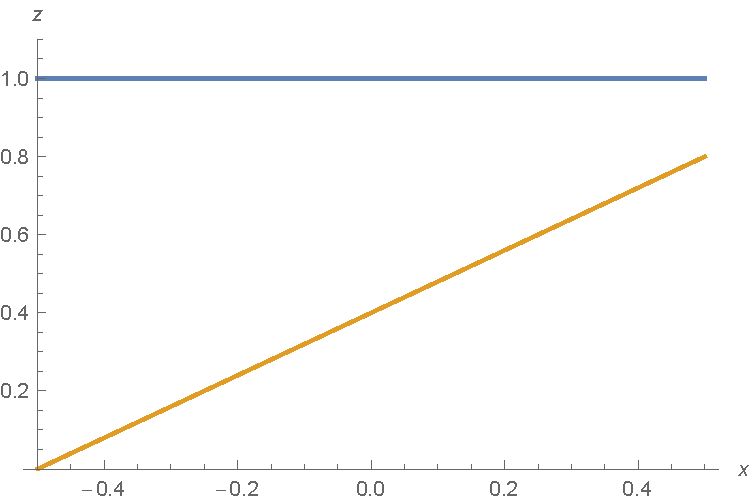
\includegraphics[width=\textwidth]{diagrams/bath-slope}
    \caption{Sloped.}
    \label{fig:bath-slope}
  \end{subfigure}
  \begin{subfigure}{0.45\textwidth}
    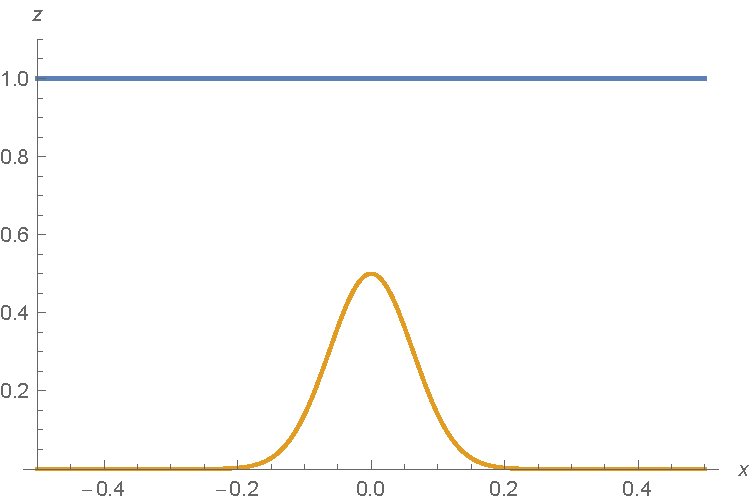
\includegraphics[width=\textwidth]{diagrams/bath-gaussian}
    \caption{Gaussian ridge.}
    \label{fig:bath-gaussian}
  \end{subfigure} \\
  \begin{subfigure}{0.45\textwidth}
    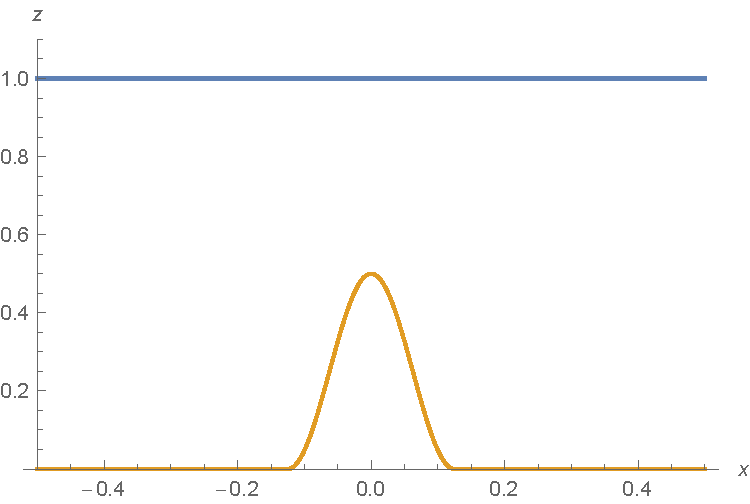
\includegraphics[width=\textwidth]{diagrams/bath-cosine}
    \caption{Cosine ridge.}
    \label{fig:bath-cosine}
  \end{subfigure}
  \begin{subfigure}{0.45\textwidth}
    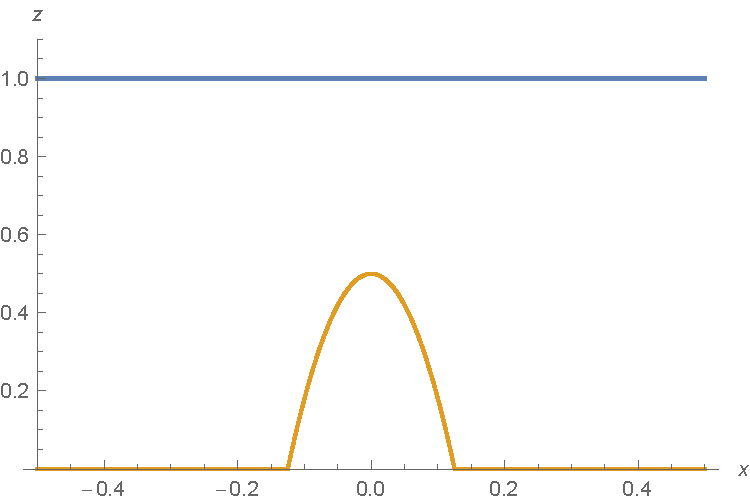
\includegraphics[width=\textwidth]{diagrams/bath-para-ridge}
    \caption{Parabolic ridge.}
    \label{fig:bath-para-ridge}
  \end{subfigure} \\
  \begin{subfigure}{0.45\textwidth}
    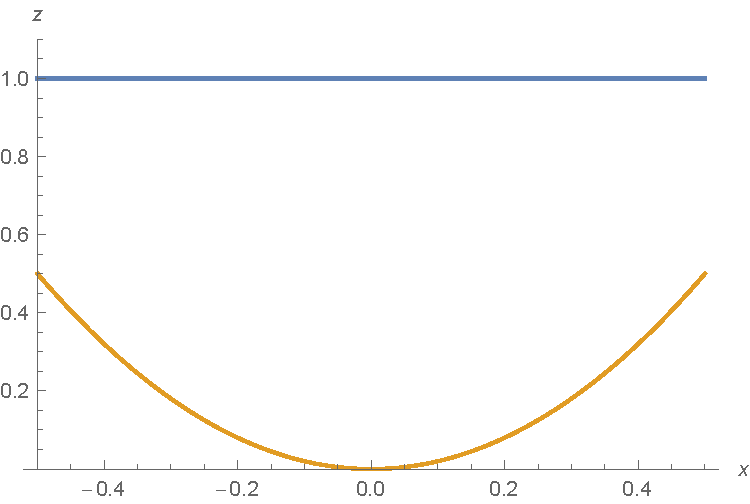
\includegraphics[width=\textwidth]{diagrams/bath-para-bowl}
    \caption{Parabolic bowl.}
    \label{fig:bath-para-bowl}
  \end{subfigure}
  \begin{subfigure}{0.45\textwidth}
    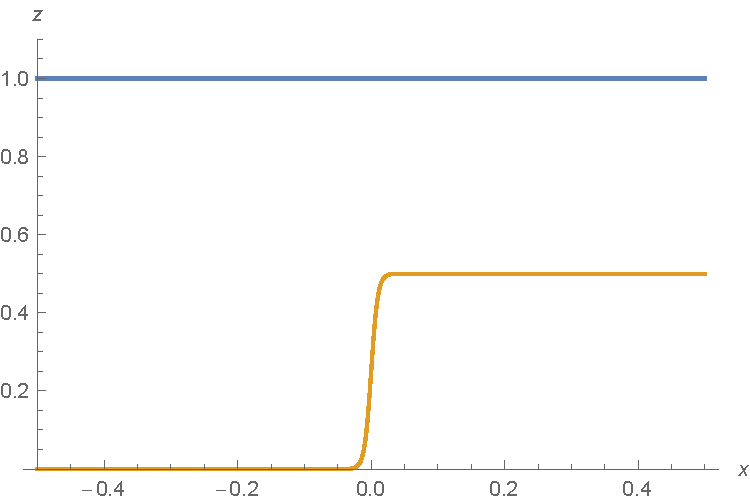
\includegraphics[width=\textwidth]{diagrams/bath-cliff}
    \caption{Cliff.}
    \label{fig:bath-cliff}
  \end{subfigure}
  \caption{Supported bathymetry profiles. Flat profile, $B = 0$, not depicted. Blue lines are still water level, $h_s = 1$, shown for scale. Orange lines are bathymetry.}
  \label{fig:bathymetries}
\end{figure}

These profiles are discretised by evaluating them on the cell edges and then averaging each cell's edge values to estimate the bathymetry at the cell centres, as required for the LeVeque solver. The other solvers do not impose any condition on the discretisation, so this scheme was used for all solvers.

The three ridge profiles may seem very similar qualitatively, but have been included for different reasons. The cosine ridge and parabolic ridge have compact support, which means that the regions of the domain affected by the bathymetry can be clearly distinguished from those which are not. Likewise, when waves travel across the ridge, it is clear at which time step the wave is first affected by the ridge. The difference between them is that the cosine ridge has a continuous derivative, while the parabola is not differentiable at $|x| = \frac{1}{8}$.

The Gaussian ridge does not have compact support but is still valuable, because this profile exactly matches the surface profile of the geostrophic equilibrium chosen (see below). By using the same profile for both water surface and bathymetry, the flux terms vanish completely (since $h$ becomes a constant), and the two source terms balance each other. This balance does not seem be addressed usually, presumably because a na\"ive unbalanced method with source split will still be well-balanced with respect to the source terms themselves (as they are computed in the same step). However, it is worth verifying whether this balance is still preserved for methods which modify how source terms are treated.

Bathymetries with non-zero slope at the domain boundaries (i.e. sloped bathymetry and the parabolic bowl) were are a good test for the chosen boundary conditions.

Independently of the bathymetry profile, one of five initial conditions can be chosen. The framework takes into account the chosen bathymetry when calculating the initial values of $\vb q$. The supported initial conditions are the following:

\begin{itemize}
  \item Still water. Defined by $h_s = 1$, $u = v = 0$. Hence, the conserved variables are chosen to be $h = 1 - B$, $hu = hv = 0$. This is shown in Figs.~\ref{fig:bathymetries}.
  \item Wave through still water. This system is mostly identical to the still water case, apart from a small perturbation near one edge of the domain, such that $h_s = 1.05$ for $|x + 0.35| < 0.05$, and $h_s = 1$ otherwise. The basic behaviour is that the perturbation separates into two waves, one of which leaves the domain to the left and one of which traverses the domain and, in particular, the bathymetry where it may be partially reflected. The exact dynamics (especially in the presence of the Coriolis term) are more complicated, but this system allows a single wave to be studied in isolation. As an example, Fig.~\ref{fig:init_wave} shows the system for the cosine ridge.
  \item Geostrophic equilibrium. The surface level is fixed at $h_s = 1 + \frac{1}{2} \exp (-128 x^2)$, such that $h$ is chosen as $h_s - B$. Furthermore, $hu = 0$ and $hv$ is determined by Eq.~\ref{eq:geo_eq}. This system requires $K \neq 0$. Figs.~\ref{fig:init_geo} show this initial condition for the flat and cliff bathymetries and several values of $K$. Note that $hv$ depends both on the bathymetry and on $K$.
  \item Wave through geostrophic equilibrium. This is essentially a linear combination of the previous two systems. First, the geostrophic equilibrium is determined, and then a height perturbation of magnitude $0.05$ is added to the interval $x \in [-0.4, -0.3]$. $hv$ is unchanged from the geostrophic equilibrium. Fig.~\ref{fig:init_geo_wave} shows the initial water level for the parabolic bowl bathymetry.
  \item Uniform flow. Defined by $h_s = 1$, $u = U$, $v = 0$, where $U$ can be freely chosen. Unless the bathymetry is flat, this is not a steady state, but will settle into a steady system for many parameter combinations. $U$ can be used to choose between subcritical, transcritical and supercritical flows, as shown in \cite{esler2005steady}. Figs.~\ref{fig:init_flow} show initial momentum for two different bathymetries --- the initial water level is indistinguishable from the still water case, and $hv$ = 0 everywhere. Note that the momentum is not uniform, because $h$ varies.
\end{itemize}

\begin{figure}
  \centering
  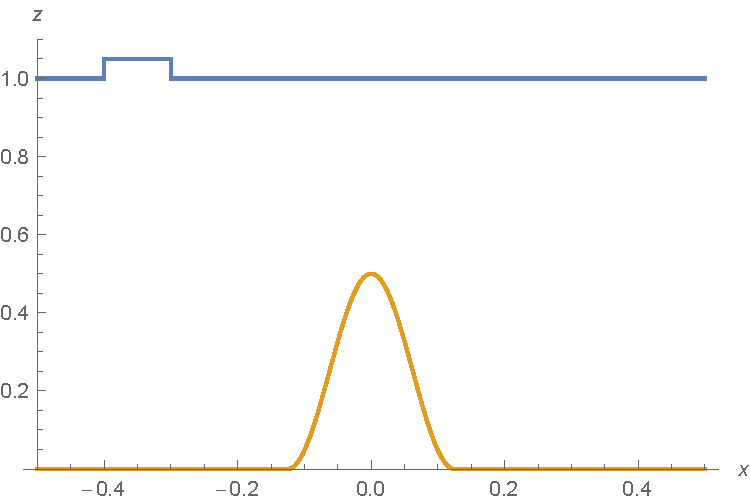
\includegraphics[width=0.45\textwidth]{diagrams/init-wave}
  \caption{Initial condition for ``wave through still water'' system and cosine bathymetry. Orange is the bathymetry profile, $B$. Blue is the initial water level, $h_s = h + B$.}
  \label{fig:init_wave}
\end{figure}

\begin{figure}
  \centering
  \begin{subfigure}{0.45\textwidth}
    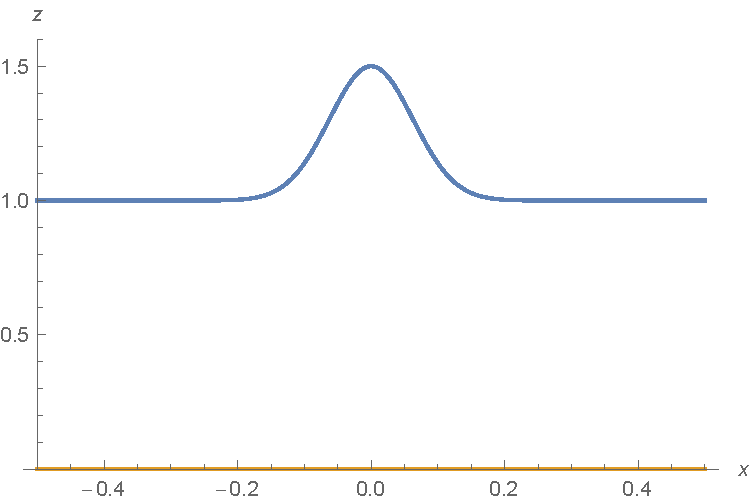
\includegraphics[width=\textwidth]{diagrams/init-geo-flat-h}
    \caption{Water level for flat bathymetry.}
    \label{fig:init-geo-flat-h}
  \end{subfigure}
  \begin{subfigure}{0.45\textwidth}
    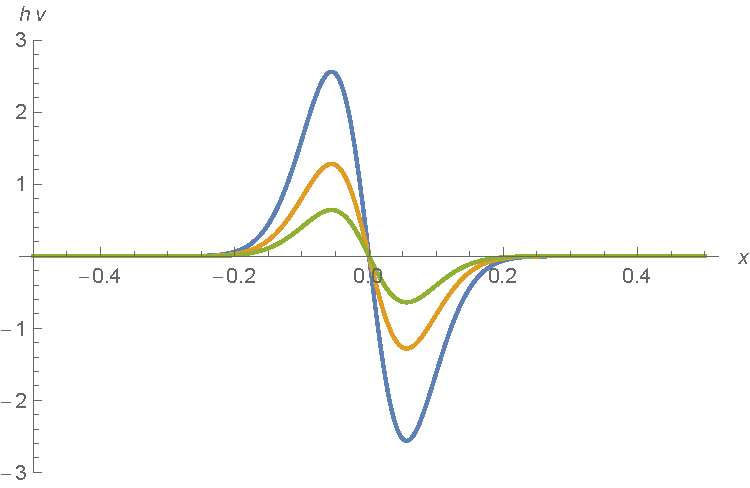
\includegraphics[width=\textwidth]{diagrams/init-geo-flat-hv}
    \caption{$y$-momentum for flat bathymetry.}
    \label{fig:init-geo-flat-hv}
  \end{subfigure} \\
  \begin{subfigure}{0.45\textwidth}
    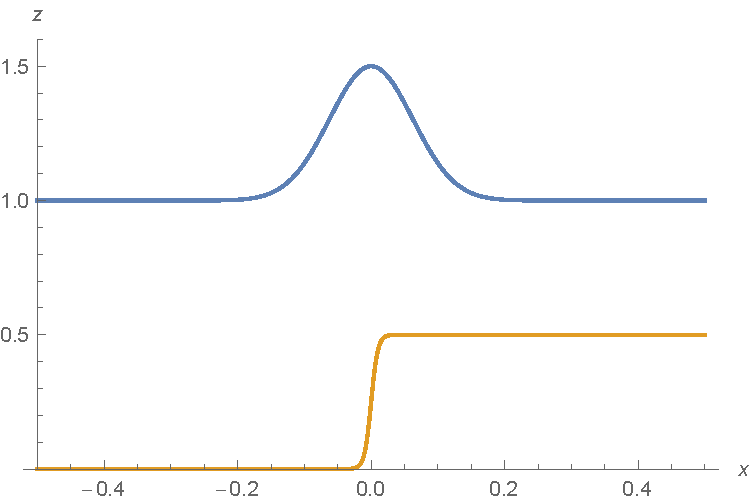
\includegraphics[width=\textwidth]{diagrams/init-geo-cliff-h}
    \caption{Water level for cliff bathymetry.}
    \label{fig:init-geo-cliff-h}
  \end{subfigure}
  \begin{subfigure}{0.45\textwidth}
    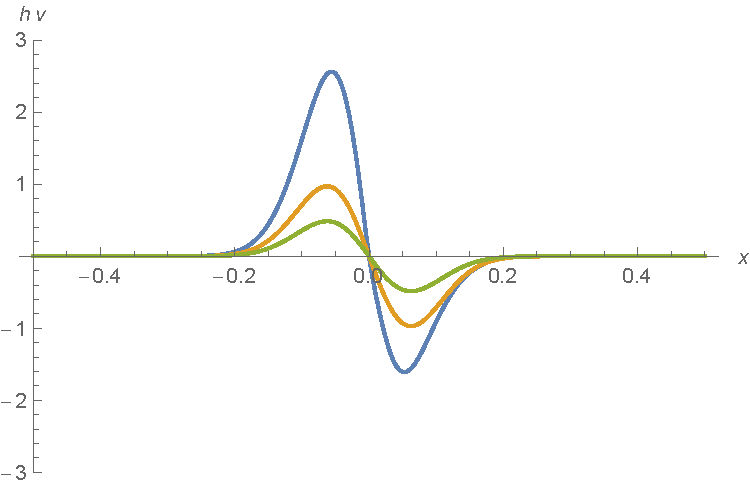
\includegraphics[width=\textwidth]{diagrams/init-geo-cliff-hv}
    \caption{$y$-momentum for cliff bathymetry.}
    \label{fig:init-geo-cliff-hv}
  \end{subfigure}
  \caption{Initial conditions for geostrophic equilibria for two bathymetry profiles. In the $hv$ plots, blue corresponds to $K = 2.5$, orange to $K = 5$ and green to $K = 10$.}
  \label{fig:init_geo}
\end{figure}

\begin{figure}
  \centering
  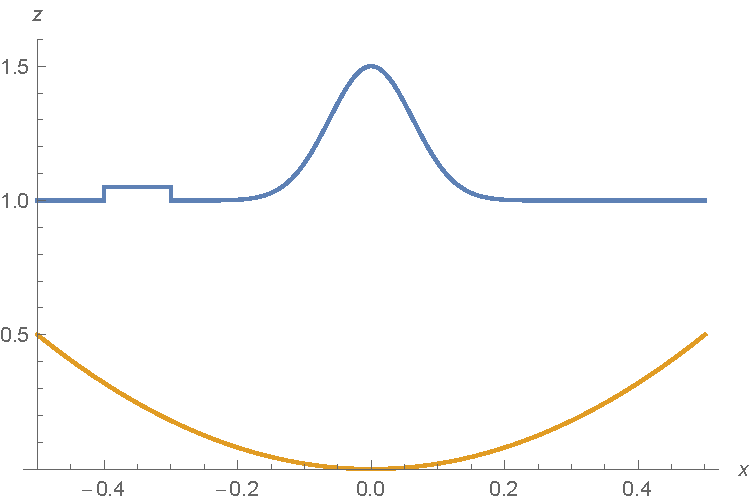
\includegraphics[width=0.45\textwidth]{diagrams/init-geo-wave}
  \caption{Initial condition for ``wave through geostrophic equilibrium'' system and parabolic bowl bathymetry. Orange is the bathymetry profile, $B$. Blue is the initial water level, $h_s = h + B$.}
  \label{fig:init_geo_wave}
\end{figure}

\begin{figure}
  \centering
  \begin{subfigure}{0.45\textwidth}
    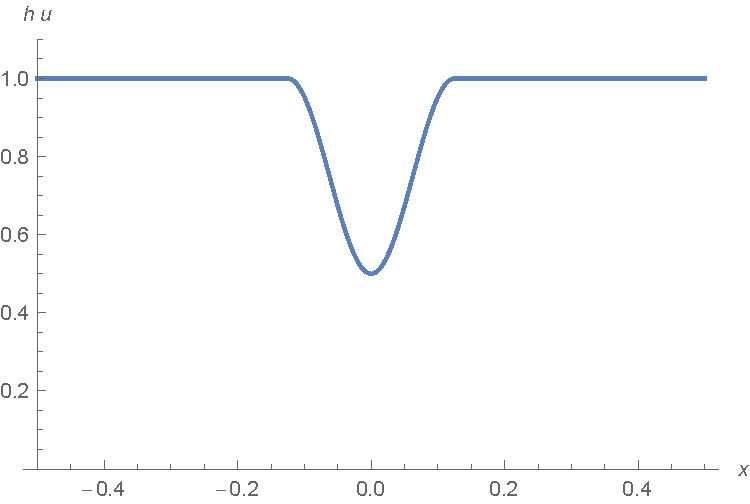
\includegraphics[width=\textwidth]{diagrams/init-steady-cosine}
    \caption{$x$-momentum for cosine ridge.}
    \label{fig:init-steady-cosine}
  \end{subfigure}
  \begin{subfigure}{0.45\textwidth}
    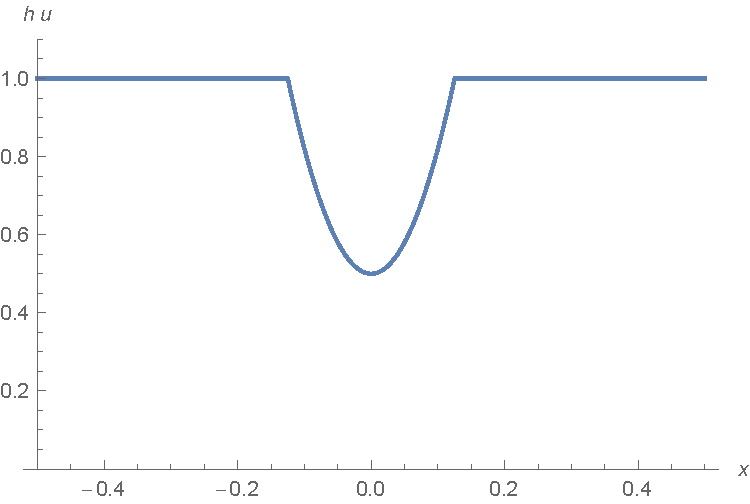
\includegraphics[width=\textwidth]{diagrams/init-steady-para}
    \caption{$x$-momentum for parabolic ridge.}
    \label{fig:init-steady-para}
  \end{subfigure}
  \caption{Initial conditions for uniform flow for two bathymetry profiles.}
  \label{fig:init_flow}
\end{figure}

\section{Notes on LeVeque Solver}
\label{sec:cubic}

As mentioned in Section~\ref{sec:leveque}, a cubic equation needs to be solved to determine the size of the new Riemann problem at the cell centres. Two different approaches have been implemented which can be chosen via a flag in the Fortran code:

\begin{itemize}
  \item As implemented by LeVeque, the Newton--Raphson method can be used to improve an initial guess. If the solution does not converge within five iterations, the attempt is aborted and a warning is printed.
  \item Alternatively, the roots can be found using an explicit formula (see \cite{press2007numerical}, pp. 178--179). However, when the discriminant is greater than $0$, this yields three real roots and one of them has to be chosen. In this case, the author's implementation chooses the root with the smallest absolute value in order to disturb the conserved variables as little as possible (and ensure that the positivity of $h$ is preserved if possible).
\end{itemize}